\documentclass[11pt,a4paper]{article}
\usepackage{notes}
\usepackage{pgfplots}

\begin{document}

%\begin{figure}[hbt]
    \centering
    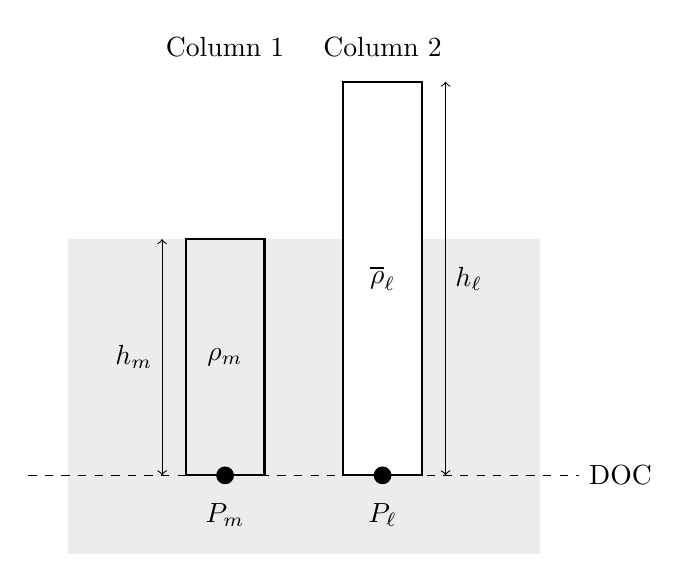
\begin{tikzpicture}[scale=1.0]

        % Asthenosphere
        \fill[gray!15] (-1.5,-1) rectangle (4.5,3);

        % Elevation difference
        \draw[<->] (-0.3,0) -- (-0.3,3) node[midway,left] {$h_m$};

        \draw[thick] (0,0) rectangle (1,3);
        \node[above] at (0.5,5.2) {Column 1};
        \draw[fill=black] (0.5,0) circle (3pt);
        \node at (0.5,1.5) {$\rho_m$};
        \node at (0.5,-0.5) {$P_m$};

        % Columns 1
        \draw[thick,fill=white] (2,0) rectangle (3,5);
        \node[above] at (2.5,5.2) {Column 2};
        \draw[fill=black] (2.5,0) circle (3pt);
        \node at (2.5,-0.5) {$P_\ell$};

        % Heights
        \draw[<->] (3.3,0) -- (3.3,5) node[midway,right] {$h_{\ell}$};

        % Compensation depth
        \draw[dashed] (-2,0) -- (5.0,0) node[right] {DOC};

        % Labels
        \node at (2.5,2.5) {$\overline{\rho}_{\ell}$};

    \end{tikzpicture}
    \caption{Schematic columns for the mantle and a column of lithosphere buoyantly supported at isostatic equilibrium. Pressure is balanced at a depth of compensation (DOC).}
    \label{fig:columns1}
\end{figure}
%\begin{figure}[hbt]
    \centering
    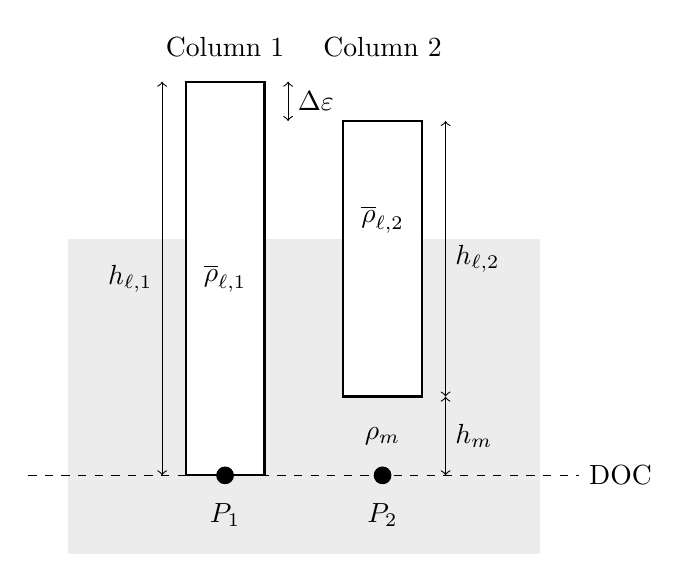
\begin{tikzpicture}[scale=1.0]

        % Asthenosphere
        \fill[gray!15] (-1.5,-1) rectangle (4.5,3);

        % Columns 1
        \draw[thick,fill=white] (0,0) rectangle (1,5);
        \node[above] at (0.5,5.2) {Column 1};
        \draw[fill=black] (0.5,0) circle (3pt);
        \node at (0.5,-0.5) {$P_1$};

        % Columns 2
        \draw[thick,fill=white] (2,1) rectangle (3,4.5);
        \node[above] at (2.5,5.2) {Column 2};
        \draw[fill=black] (2.5,0) circle (3pt);
        \node at (2.5,-0.5) {$P_2$};

        % Heights
        \draw[<->] (-0.3,0) -- (-0.3,5) node[midway,left] {$h_{\ell,1}$};
        \draw[<->] (3.3,0) -- (3.3,1) node[midway,right] {$h_m$};
        \draw[<->] (3.3,1) -- (3.3,4.5) node[midway,right] {$h_{\ell,2}$};
        \draw[<->] (1.3,4.5) -- (1.3,5) node[midway,right] {$\Delta\varepsilon$};

        % Compensation depth
        \draw[dashed] (-2,0) -- (5,0) node[right] {DOC};

        % Labels
        \node at (0.5,2.5) {$\overline{\rho}_{\ell,1}$};
        \node at (2.5,3.25) {$\overline{\rho}_{\ell,2}$};
        \node at (2.5,0.5) {$\rho_m$};

    \end{tikzpicture}
    \caption{Schematic lithospheric columns in isostatic equilibrium. Pressure is balanced at a common depth (DOC), while surface elevations differ due to variations in integrated buoyancy of each column.}
    \label{fig:columns2}
\end{figure}
%
\begin{figure}[hbtp]
    \centering
    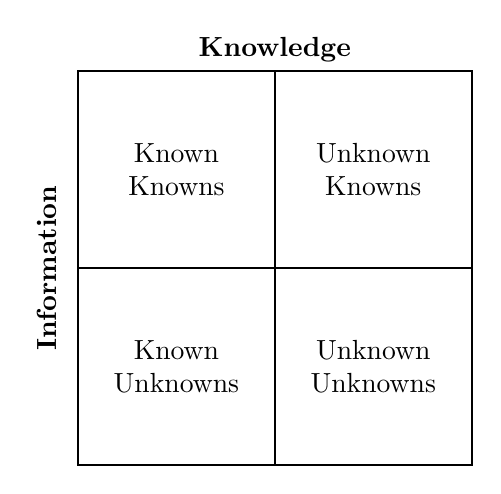
\begin{tikzpicture}[scale=1, every node/.style={align=center}]
        % Axes
        \draw[-, thick] (-2.5,0) -- (2.5,0);
        \node[rotate=90] at (-2.9, 0) {\textbf{Information}};
        \draw[-, thick] (0,-2.5) -- (0,2.5);
        \node[above] at (0, 2.5) {\textbf{Knowledge}};

        % Quadrants
        \draw[thick] (-2.5,-2.5) rectangle (2.5,2.5);

        % Labels
        \node at (-1.25,1.25) {Known\\ Knowns};
        \node at (-1.25,-1.25) {Known\\ Unknowns};
        \node at (1.25,1.25){Unknown\\ Knowns};
        \node at (1.25,-1.25){Unknown\\ Unknowns};

    \end{tikzpicture}
    \caption{Conceptual diagram, now called the Rumsfeld Matrix, can be used to describing the relationship between knowledge of a system and its properties.}
    \label{fig:rumsfeld}
\end{figure}

%\begin{tikzpicture}
\begin{axis}[
    xlabel={$m$},
    ylabel={$\Phi(m)$},
    axis lines=middle,
    domain=-2:3,
    samples=100,
]
% nonlinear function
\addplot[blue, thick] {(x-1)^2 + 0.3*sin(deg(3*x))};

% quadratic approximation (schematic)
\addplot[red, dashed, domain=-1.5:1] {0.5*(x+0.5)^2 + 1};

% lines
\addplot[dotted] coordinates {(-1,0) (-1,5)};
\addplot[dotted] coordinates {(1,0) (1,3)};

\node at (axis cs:-1,4) {$m_i$};
\node at (axis cs:1,2.5) {$m_{i+1}$};

\end{axis}
\end{tikzpicture}

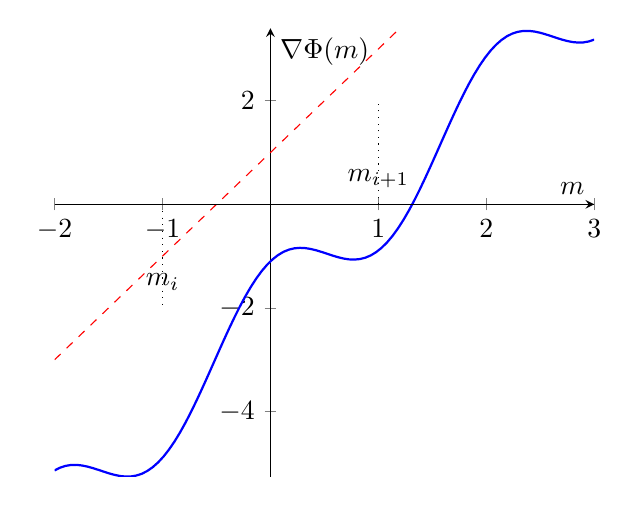
\begin{tikzpicture}
\begin{axis}[
    xlabel={$m$},
    ylabel={$\nabla \Phi(m)$},
    axis lines=middle,
    domain=-2:3,
    samples=100,
]
% gradient curve (schematic)
\addplot[blue, thick] {2*(x-1) + 0.9*cos(deg(3*x))};

% tangent line
\addplot[red, dashed, domain=-2:1.2] {-1 + 2*(x+1)};

% horizontal axis
\addplot[black] coordinates {(-2,0) (3,0)};

% verticals
\addplot[dotted] coordinates {(-1,0) (-1,-2)};
\addplot[dotted] coordinates {(1,0) (1,2)};

\node at (axis cs:-1,-1.5) {$m_i$};
\node at (axis cs:1,0.5) {$m_{i+1}$};

\end{axis}
\end{tikzpicture}
\[
    6\underbrace{\ce{(Mg,Fe)2SiO4}}_{\text{olivine}} + 7\ce{H2O} \rightarrow
    3\underbrace{\ce{(Mg,Fe)3(Si_2O_5(OH))4}}_{\text{serpentine}} +
    \underbrace{\ce{Fe3O4}}_{\text{magnetite}} + \ce{H2} .
\]
Another example includes the exsolution of titanomagnetite during cooling can change magnetic minerals,
\[
    \underbrace{\ce{Fe_{3-x}Ti_xO4}}_{\text{titanomagnetite}} \rightarrow
    \underbrace{\ce{Fe3O4}}_{\text{magnetite}} +
    \underbrace{\ce{FeTiO3}}_{\text{ilmenite}} + \text{intermediate~spinels} .
\]
Near earth's surface, oxidation to hematite may weaken or modify magnetic signals
\[
    4\underbrace{\ce{Fe3O4}}_{\text{magnetite}} + \ce{O2} \rightarrow
    6\underbrace{\ce{Fe2O3}}_{\text{hematite}} .
\]

\end{document}